\section{Langkah-Langkah Percobaan}
\begin{enumerate}
	\item Reset Router untuk membersihkan sisa pengaturan dari praktikum sebelumnya\\
	\includegraphics[width=0.4\textwidth]{p4/img/restart.jpg}
	\item Login ke Router di winbox \\
	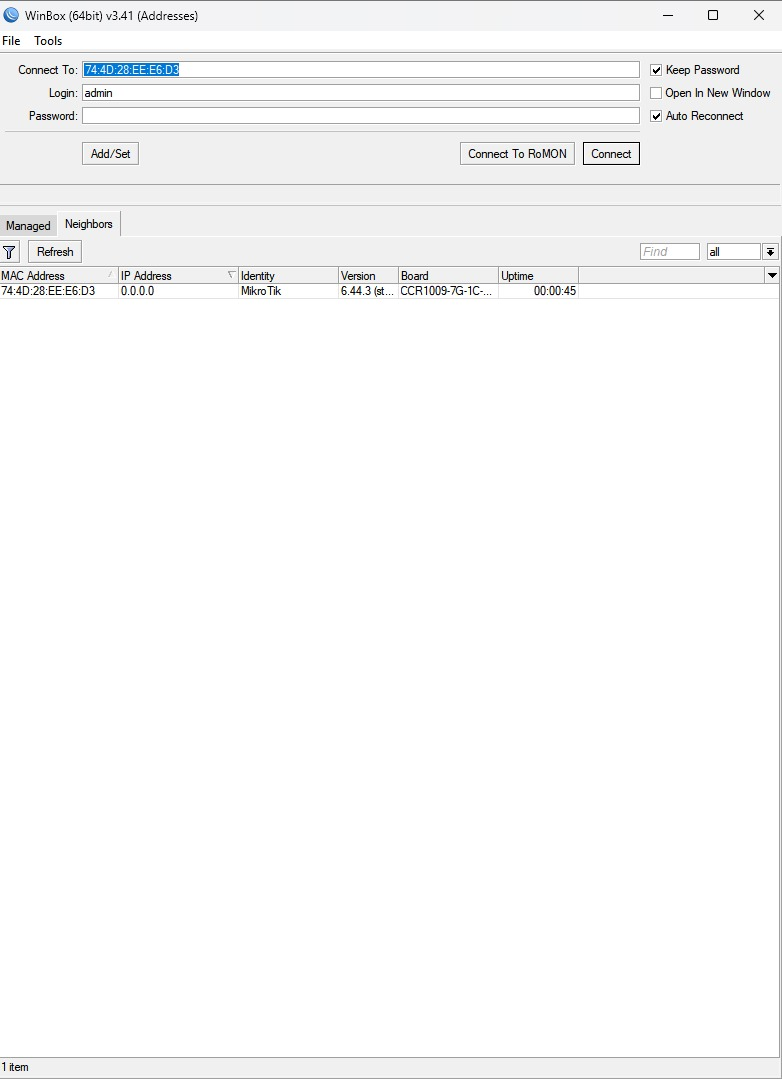
\includegraphics[width=0.4\textwidth]{p4/img/login.jpg}
	\item Konfigurasi DHCP Client pada Router di menu IP > DHCP Client\\
	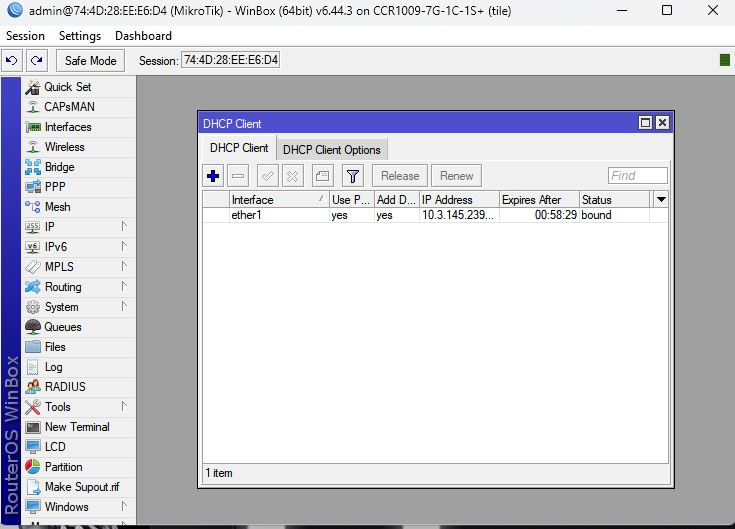
\includegraphics[width=0.4\textwidth]{p4/img/DHCP2.jpg}
	\item Konfigurasi NAT\\
	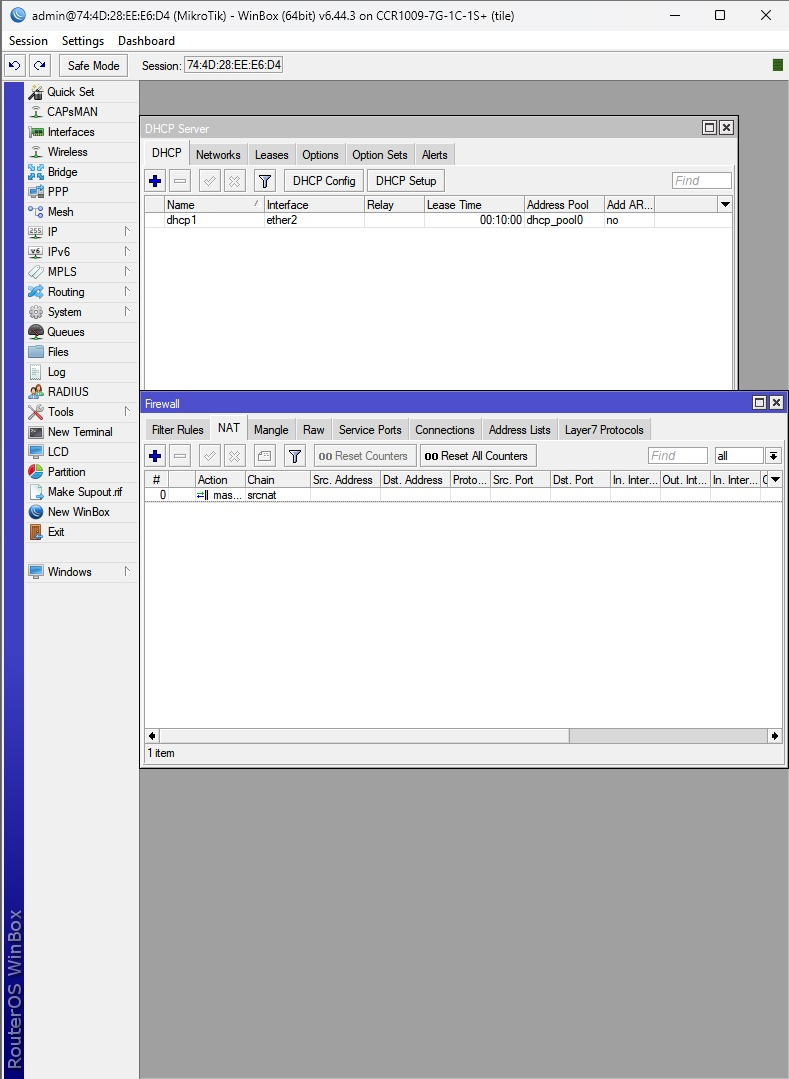
\includegraphics[width=0.4\textwidth]{p4/img/NAT.jpg}
	\item uji ping 8.8.8.8 di PC1\\
	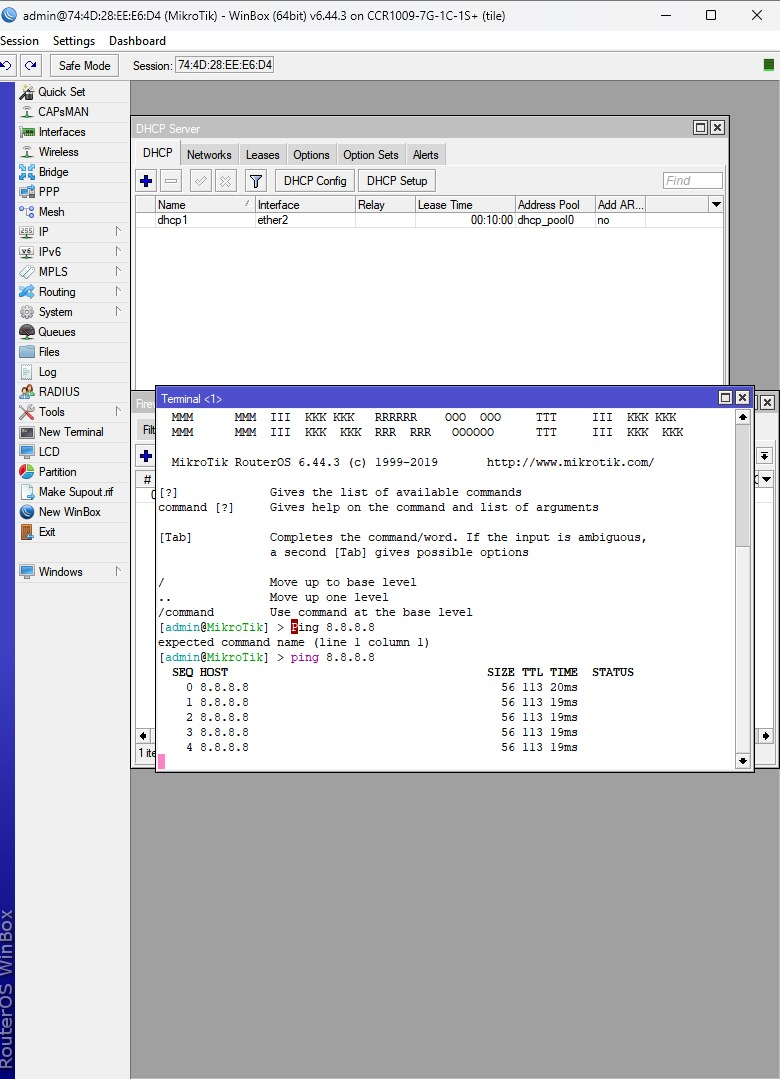
\includegraphics[width=0.4\textwidth]{p4/img/8888_p1.jpg}
	\item Konfigurasi Firewall\\
	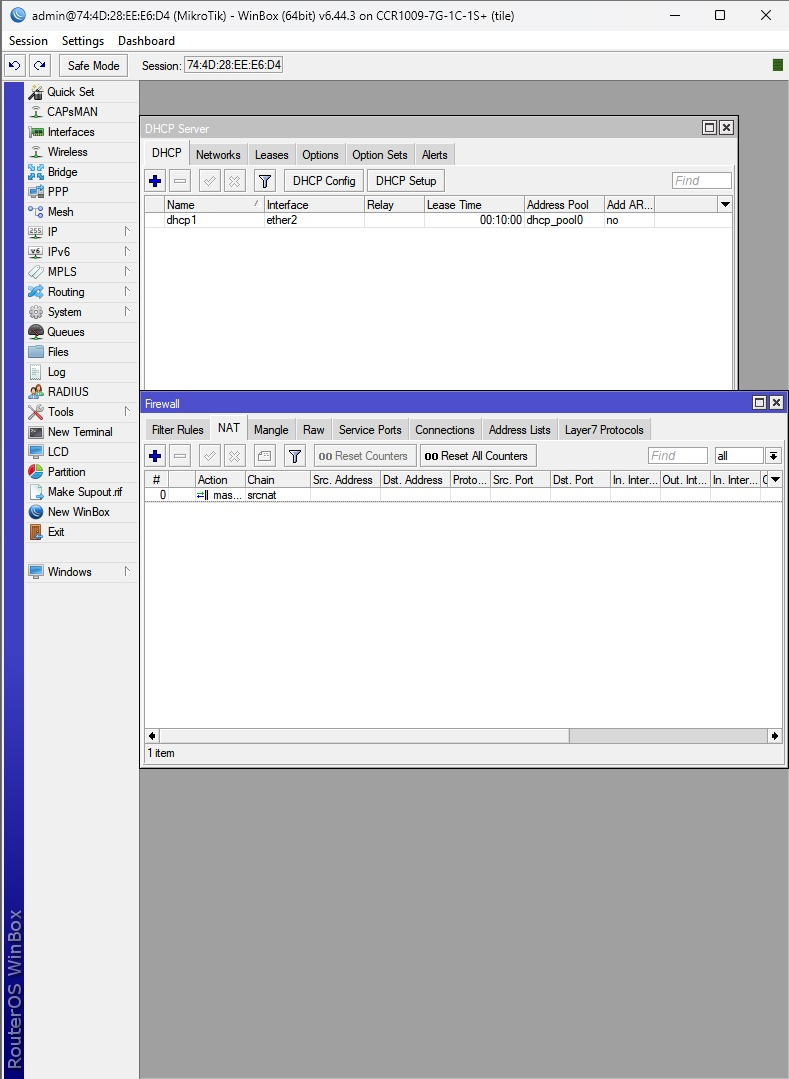
\includegraphics[width=0.4\textwidth]{p4/img/firewall_set.jpg}
	\item Blokir ICMP\\
	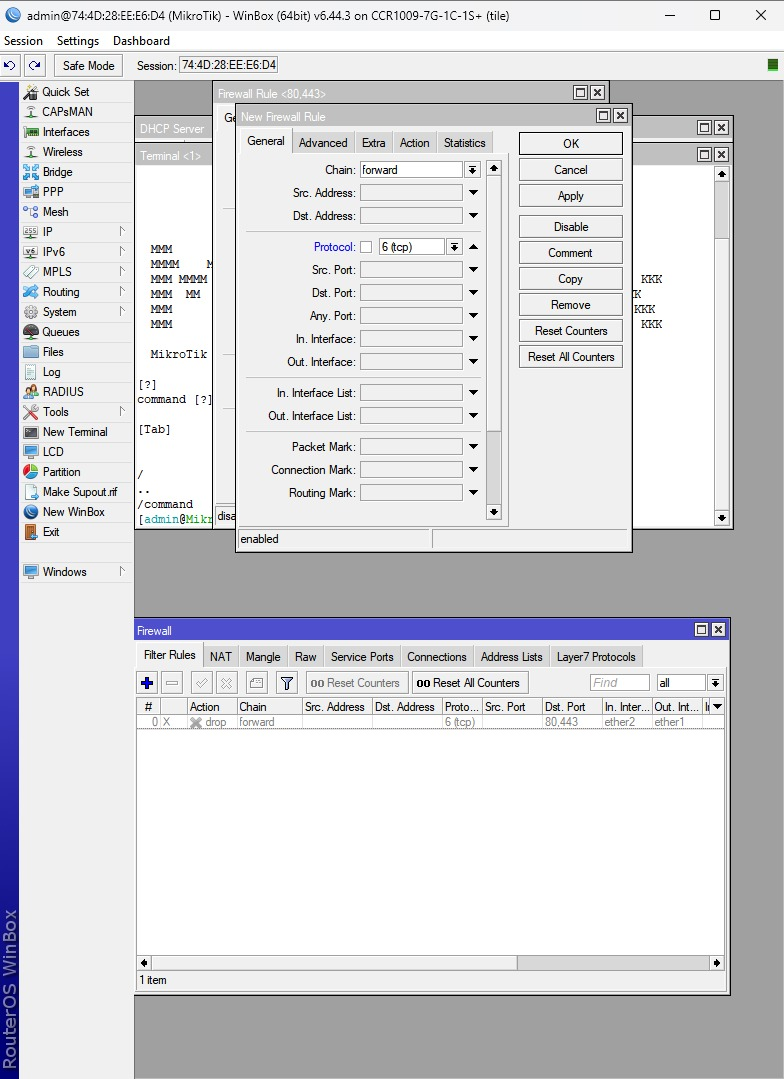
\includegraphics[width=0.4\textwidth]{p4/img/block1.jpg}
	\item Blokir Akses Situs Speedtest\\
	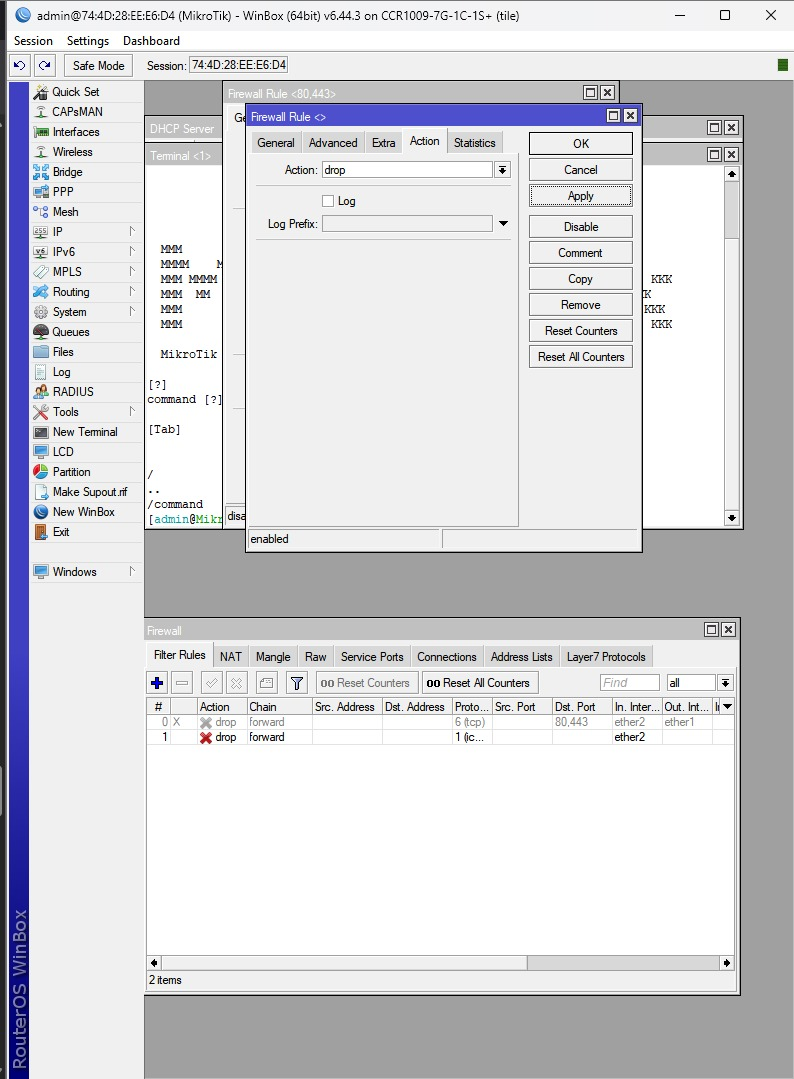
\includegraphics[width=0.4\textwidth]{p4/img/block2.jpg}
	\item Konfigurasi Router 2 sebagai Bridge\\
	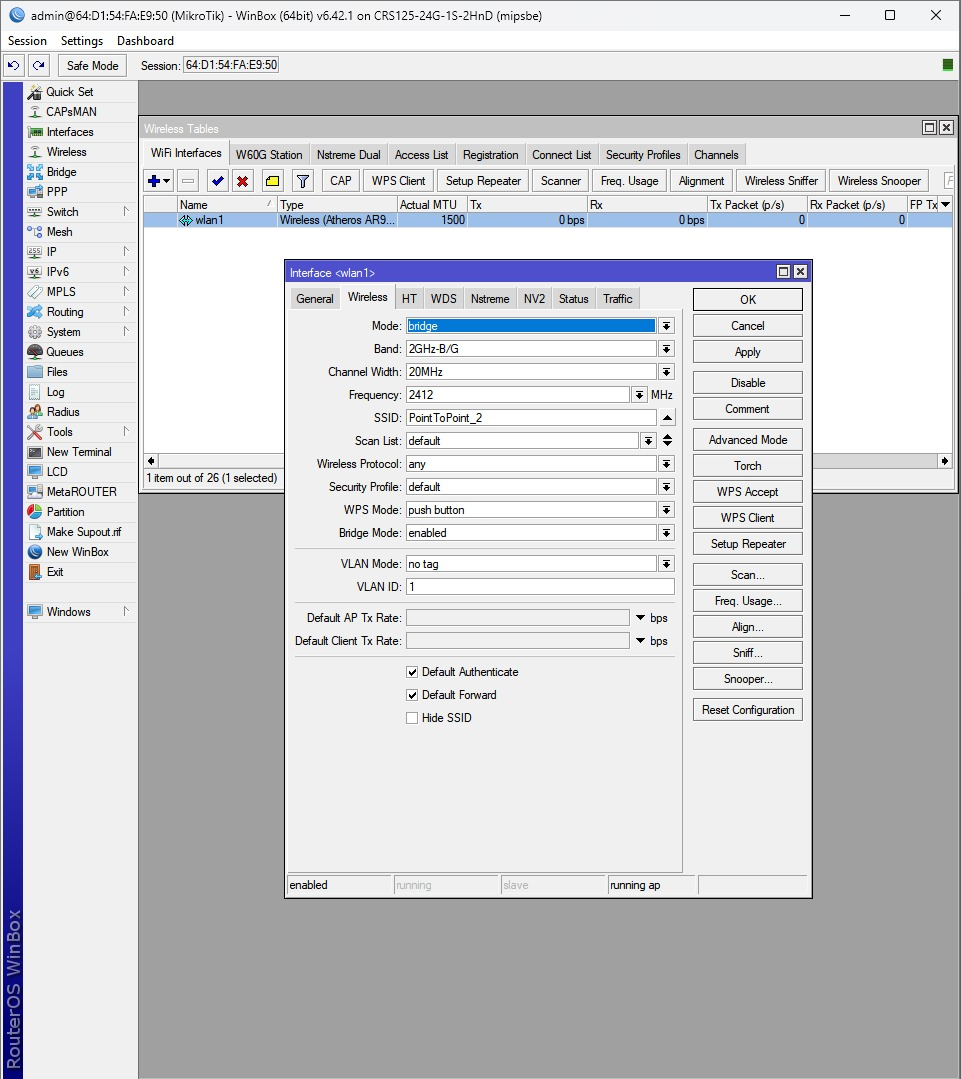
\includegraphics[width=0.4\textwidth]{p4/img/bridge.jpg}
	\item Uji Ping 8.8.8.8 dan uji akses website speedtest pada PC2\\
	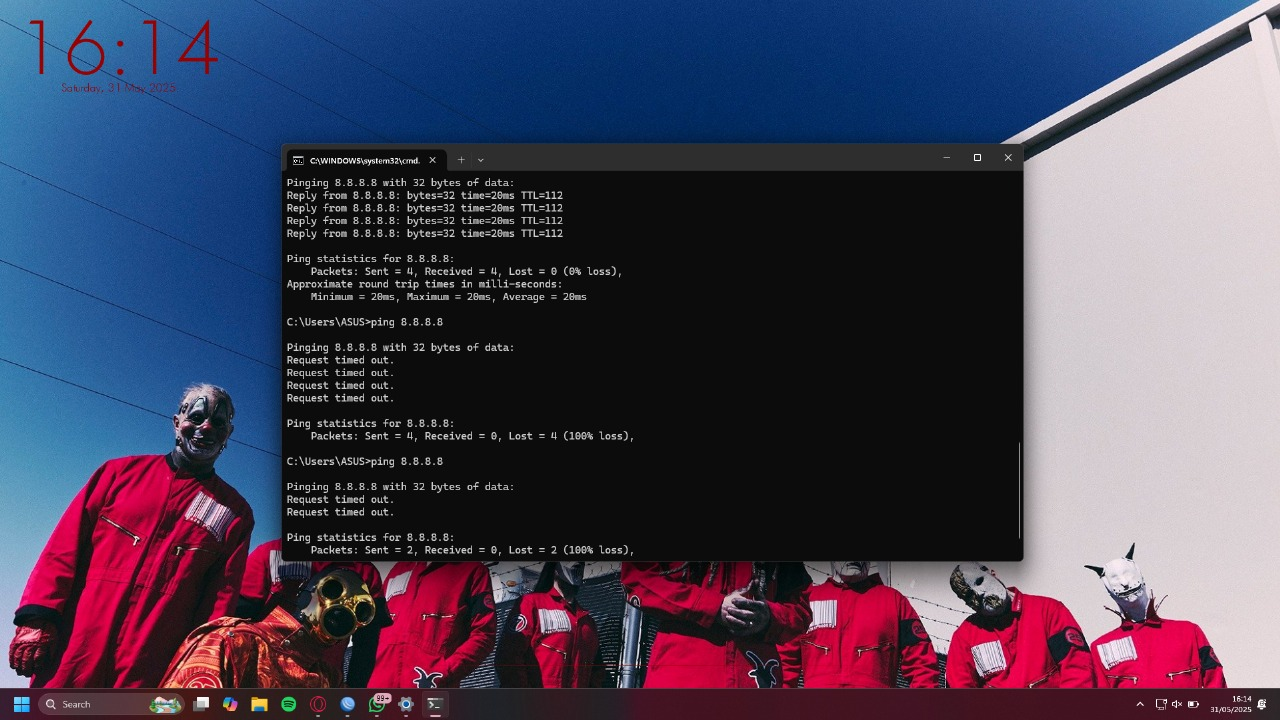
\includegraphics[width=0.4\textwidth]{p4/img/ping_blocked.jpg}
	\item Buka blokir ICMP \& Akses Situs Speedtest di Firewall\\
	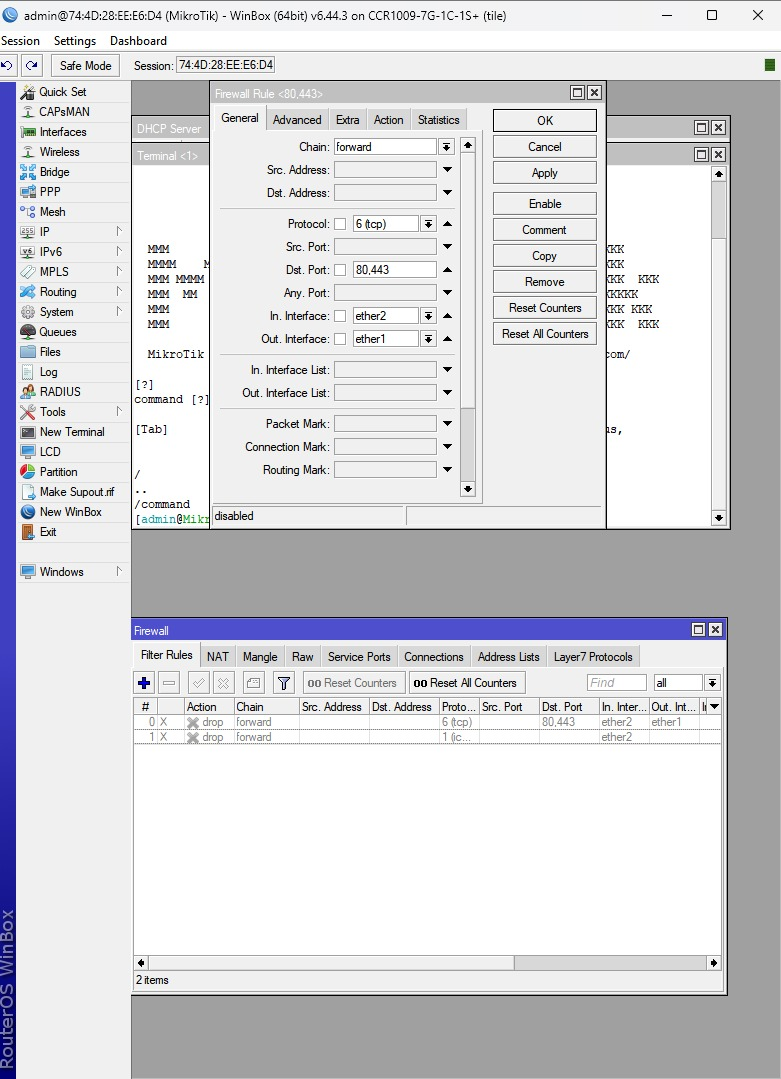
\includegraphics[width=0.4\textwidth]{p4/img/unblock.jpg}
	\item Uji lagi Ping 8.8.8.8 dan uji akses website Speedtest pada PC2\\
	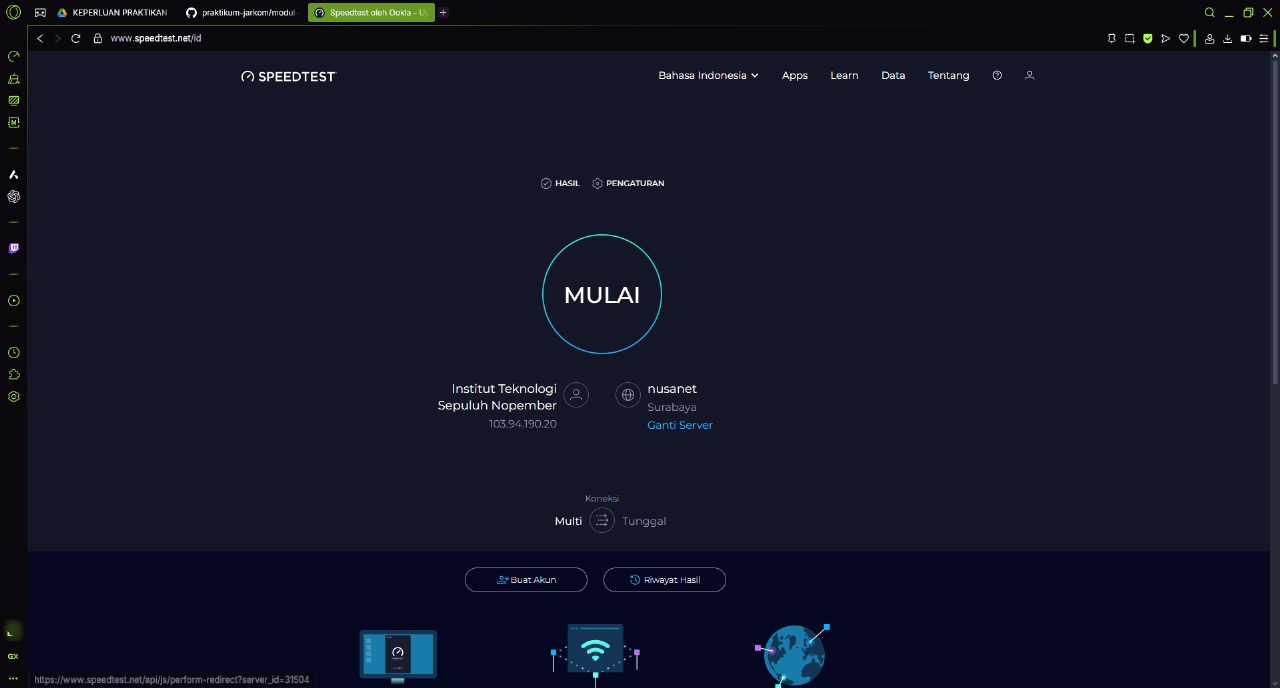
\includegraphics[width=0.4\textwidth]{p4/img/spdtst.jpg}
\end{enumerate}
\section{Analisis Hasil Percobaan}
Pada praktikum ini membahas tentang NAT dan Firewall. Pada percobaan pertama adalah pengaturan NAT, setelah NAT diatur kemudian diatur firewall. Terdapat 2 tahap setelah NAT dan Firewall diatur. Yang pertama adalah melakukan blokir untuk ping 8.8.8.8 dan membukan speedtest. Saat diblokir, ketika PC2 mencoba melakukan ping ke 8.8.8.8 didapatkan hasil request timed out, dan ketika dicoba membuka speedtest.net akan terus mengalami loading. Kemudian ketika blokir dibuka dan diperbolehkan, maka ketika PC2 mencoba kembali melakukan ping ke 8.8.8.8 maka didapatkan tanggapan dan ping berhasil, serta ketika mecoba mengakses speedtest.net, PC2 dapat membuka speedtest.net dengan normal.
\section{Hasil Tugas Modul}
Berikut adalah gambaran topologi jaringan yang telah dibangun menggunakan Cisco Packet Tracer. Topologi ini terdiri dari satu router, satu switch, tiga PC (LAN), dan satu server (publik/internet).
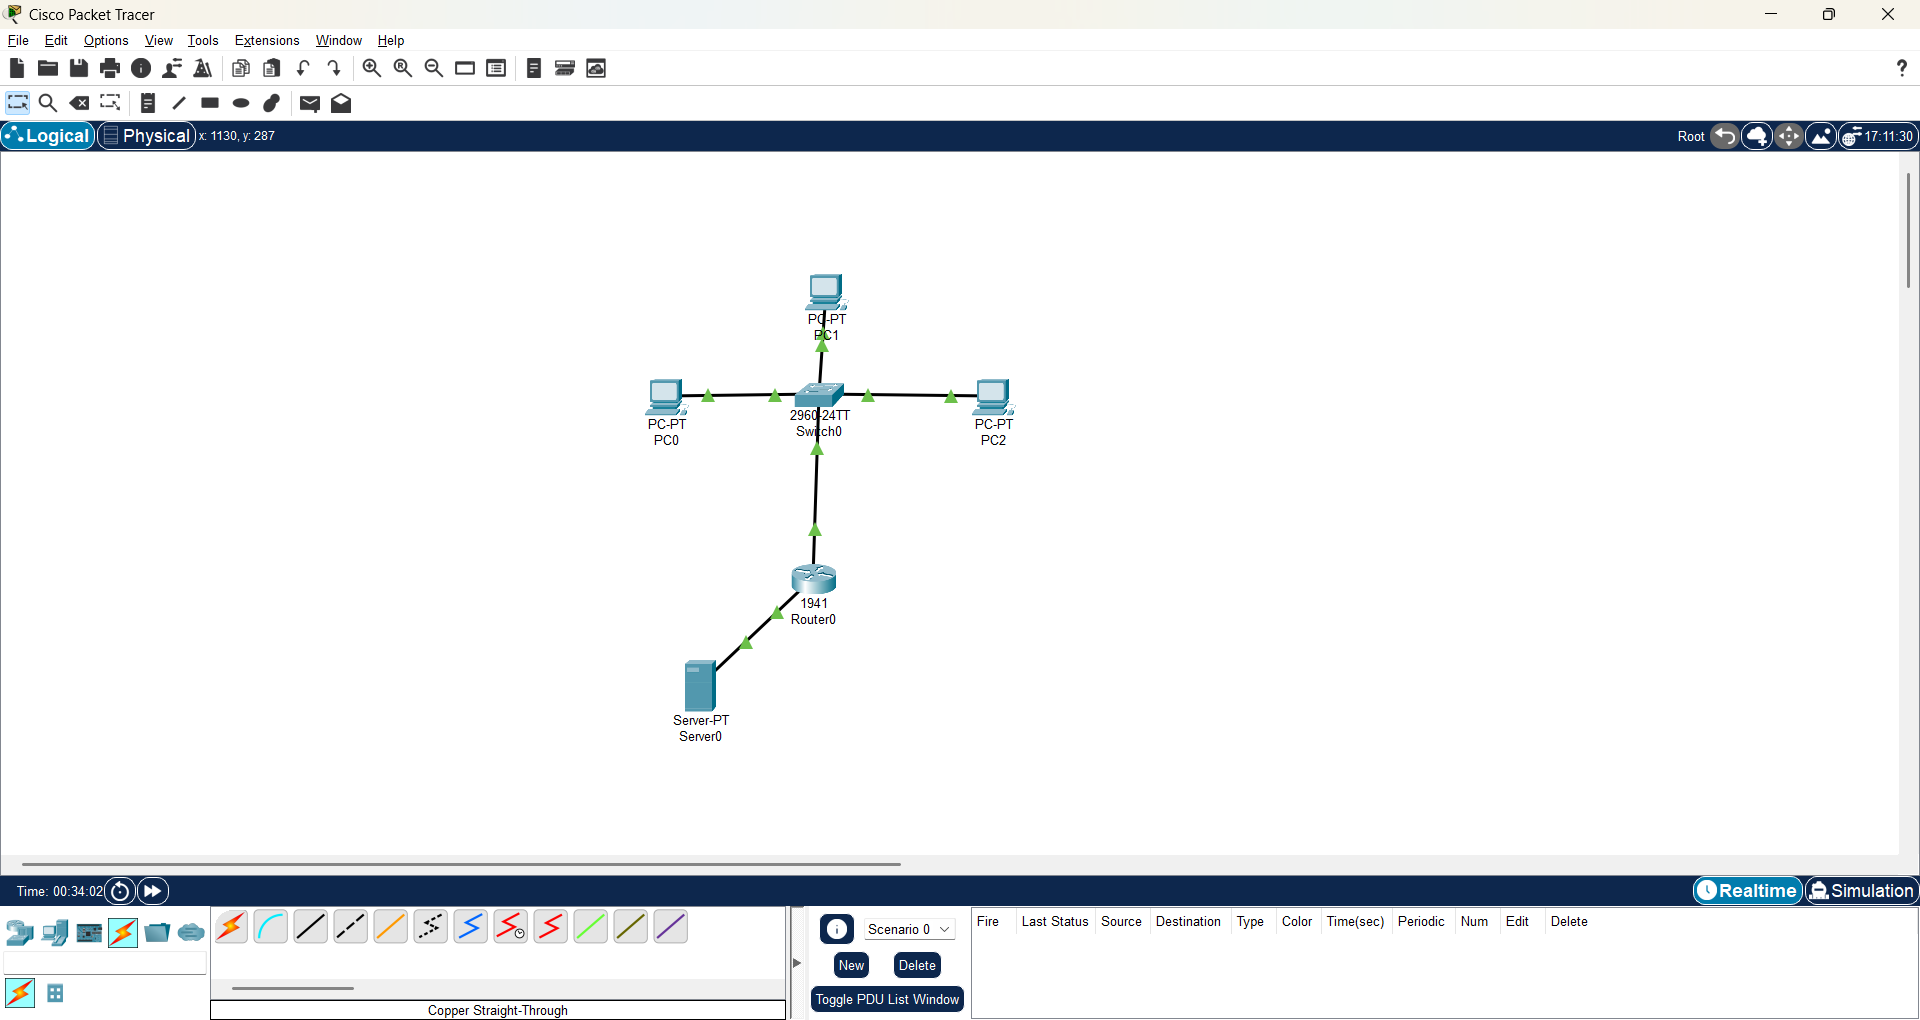
\includegraphics[width=0.7\textwidth]{p4/img/topologi.png}\\
Dari hasil Topologi diatas, dilakukan set up NAT\\
Setelah NAT diset up kemudian dilakukan percobaan ping dari PC ke Server\\
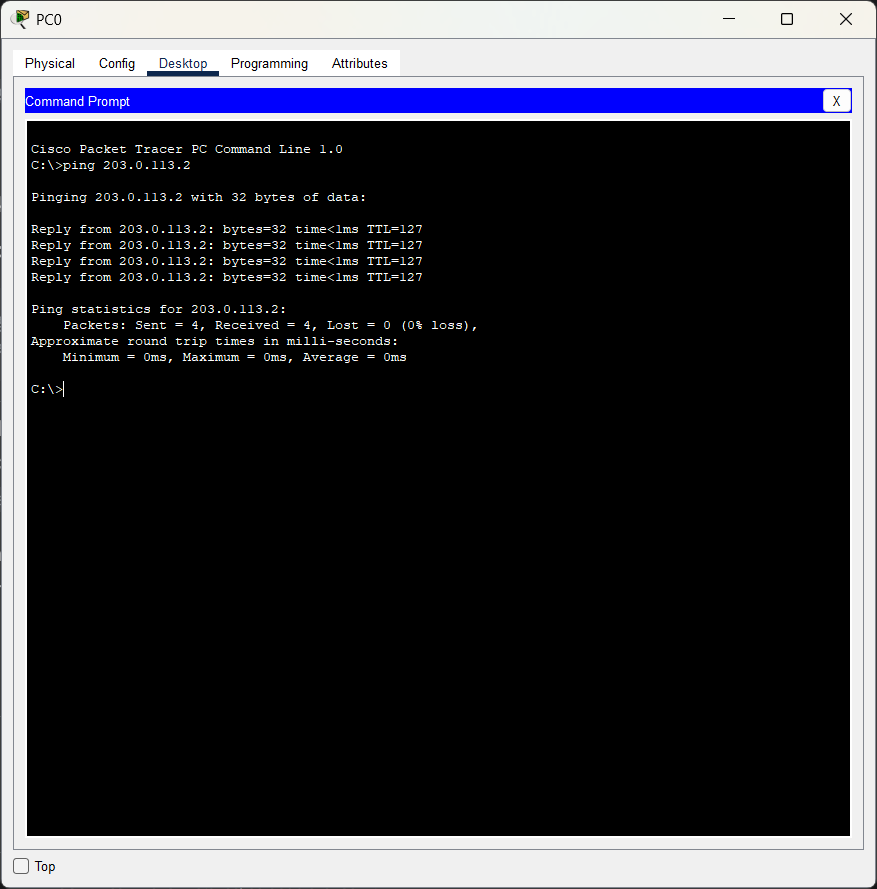
\includegraphics[width=0.4\textwidth]{p4/img/tumod1.png}
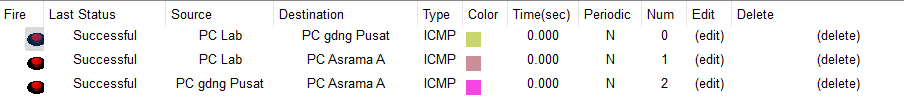
\includegraphics[width=0.4\textwidth]{p4/img/tumod2.png}\\
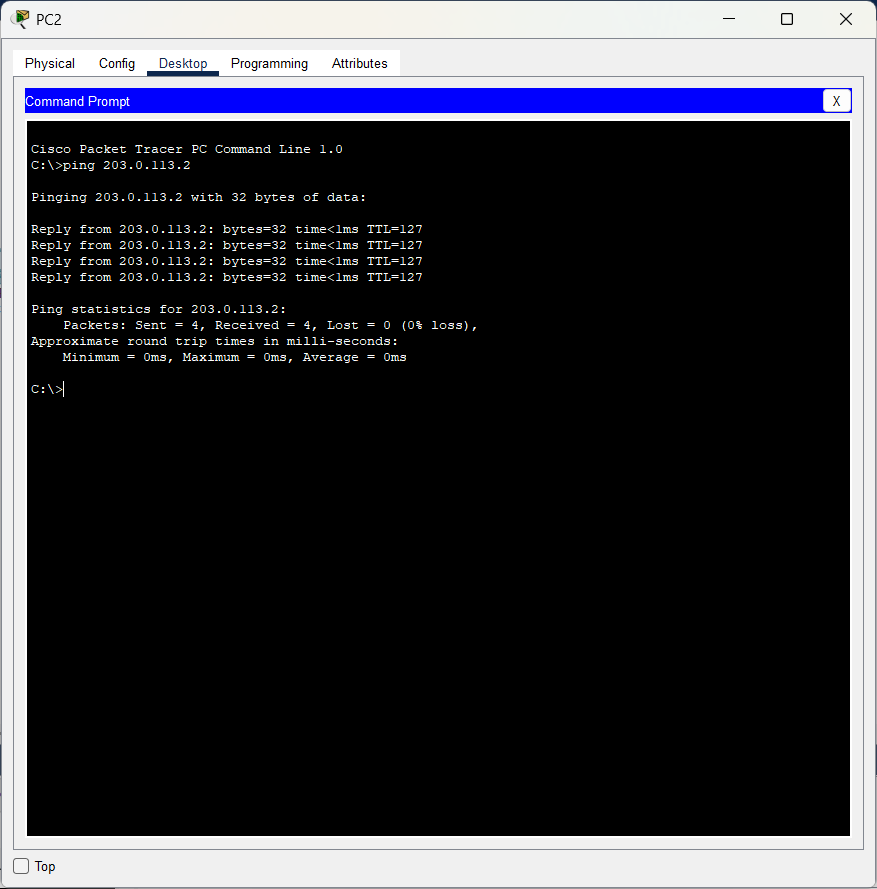
\includegraphics[width=0.4\textwidth]{p4/img/tumod3.png}\\
Diatas adalah hasil tes ping dari PC ke server setelah NAT berhasil di atur
Kemudian dibuat Firewall yang memblokir semua PC kecuali PC0 untuk melakukan ping ke server
setelah diatur maka hasil dari pengaturan ini akan menjadi\\
\includegraphics[width=0.7\textwidth]{p4/img/Firewall.png}\\
dimana diberi permit untuk IP PC0 192.168.1.11 namun semua ip lain pada network 192.168.1.0 diblokir.
Ketika dicoba ping dari PC0 ke server dan didapatkan sebagai berikut\\
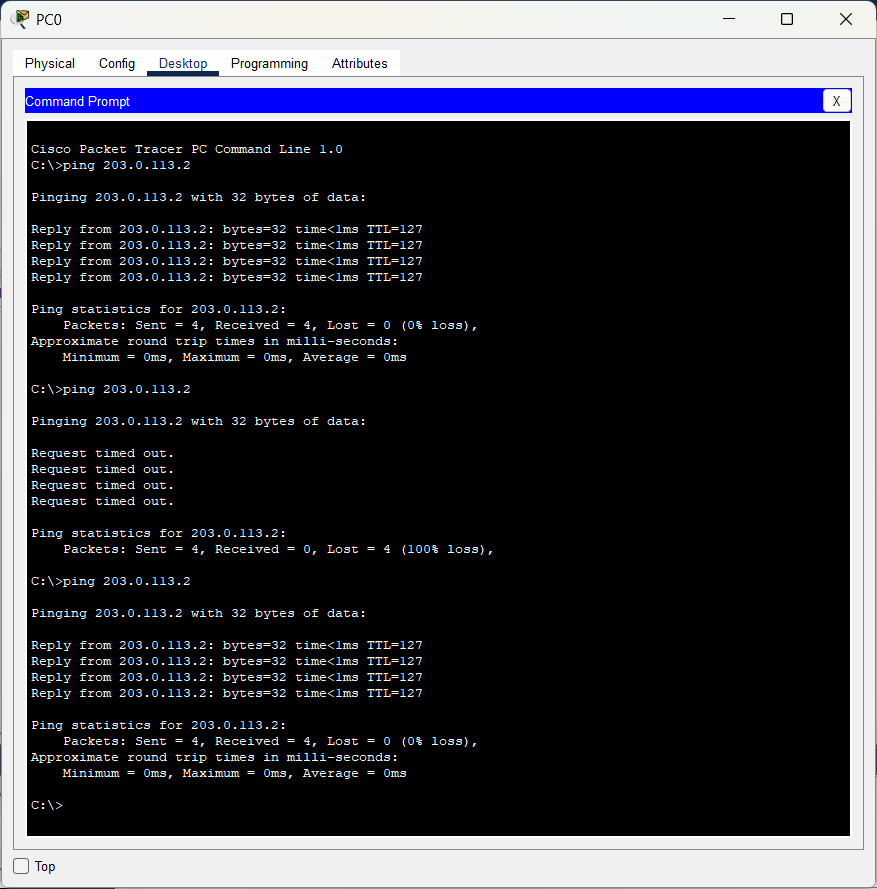
\includegraphics[width=0.7\textwidth]{p4/img/tumod4.png}\\
sementara itu untuk PC1 dan PC2\\
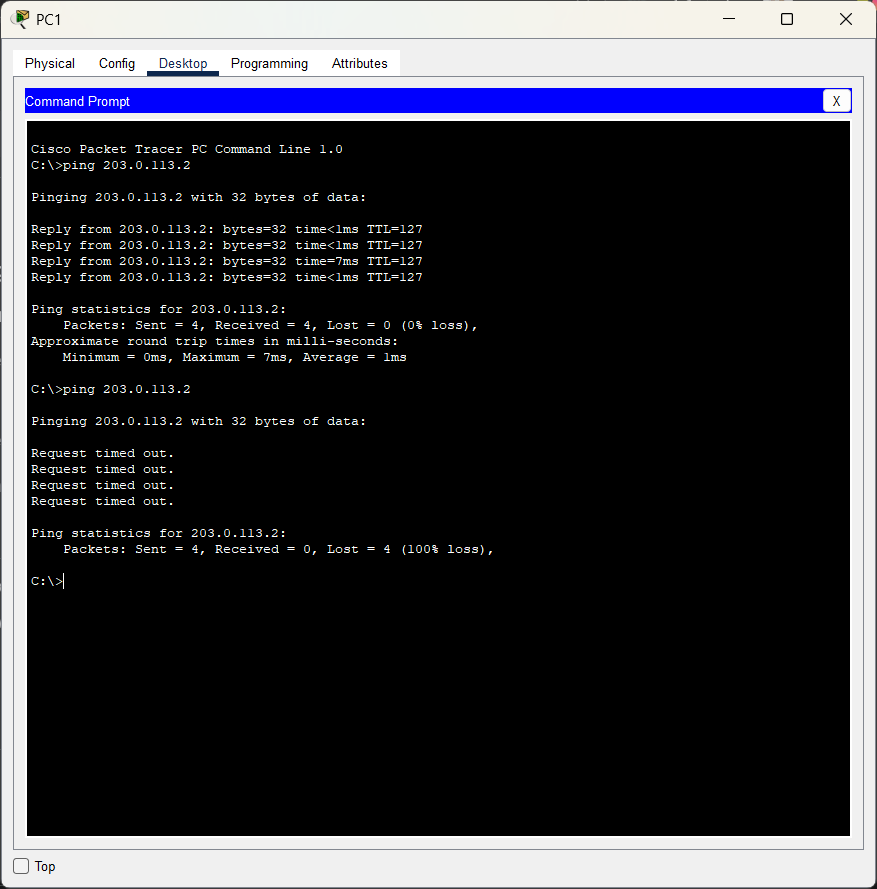
\includegraphics[width=0.4\textwidth]{p4/img/tumod5.png}
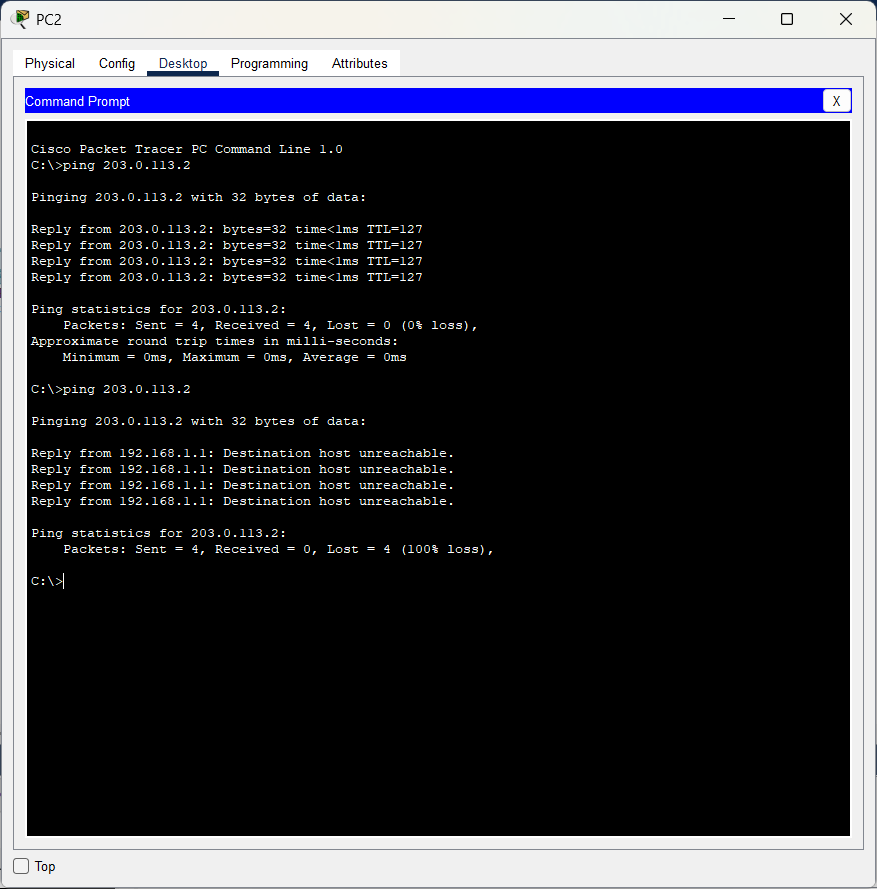
\includegraphics[width=0.4\textwidth]{p4/img/tumod6.png}\\
yang menandakan bahwa PC1 dan PC2 terblokir dari melakukan ping ke server.
\section{Kesimpulan}
Dari praktikum yang telah dilakukan, dapat disimpulkan bahwa penggunaan NAT membuat kita dapat menggunakan 1 IP address publik untuk beberapa perangkat sehingga membantu dalam pembagian IP. Kemudian bahwa pentingnya Firewall yang dapat membantu memfilter data yang diterima oleh perangkat ketika terhubung dalam jaringan. Selain itu, Firewall dapan digunakan untuk memblokir website atau konten berbahaya yang menjaga keamanan perangkat.

\section{Lampiran}
\subsection{Dokumentasi saat praktikum}
dokumentasi topologi saat praktikum\\
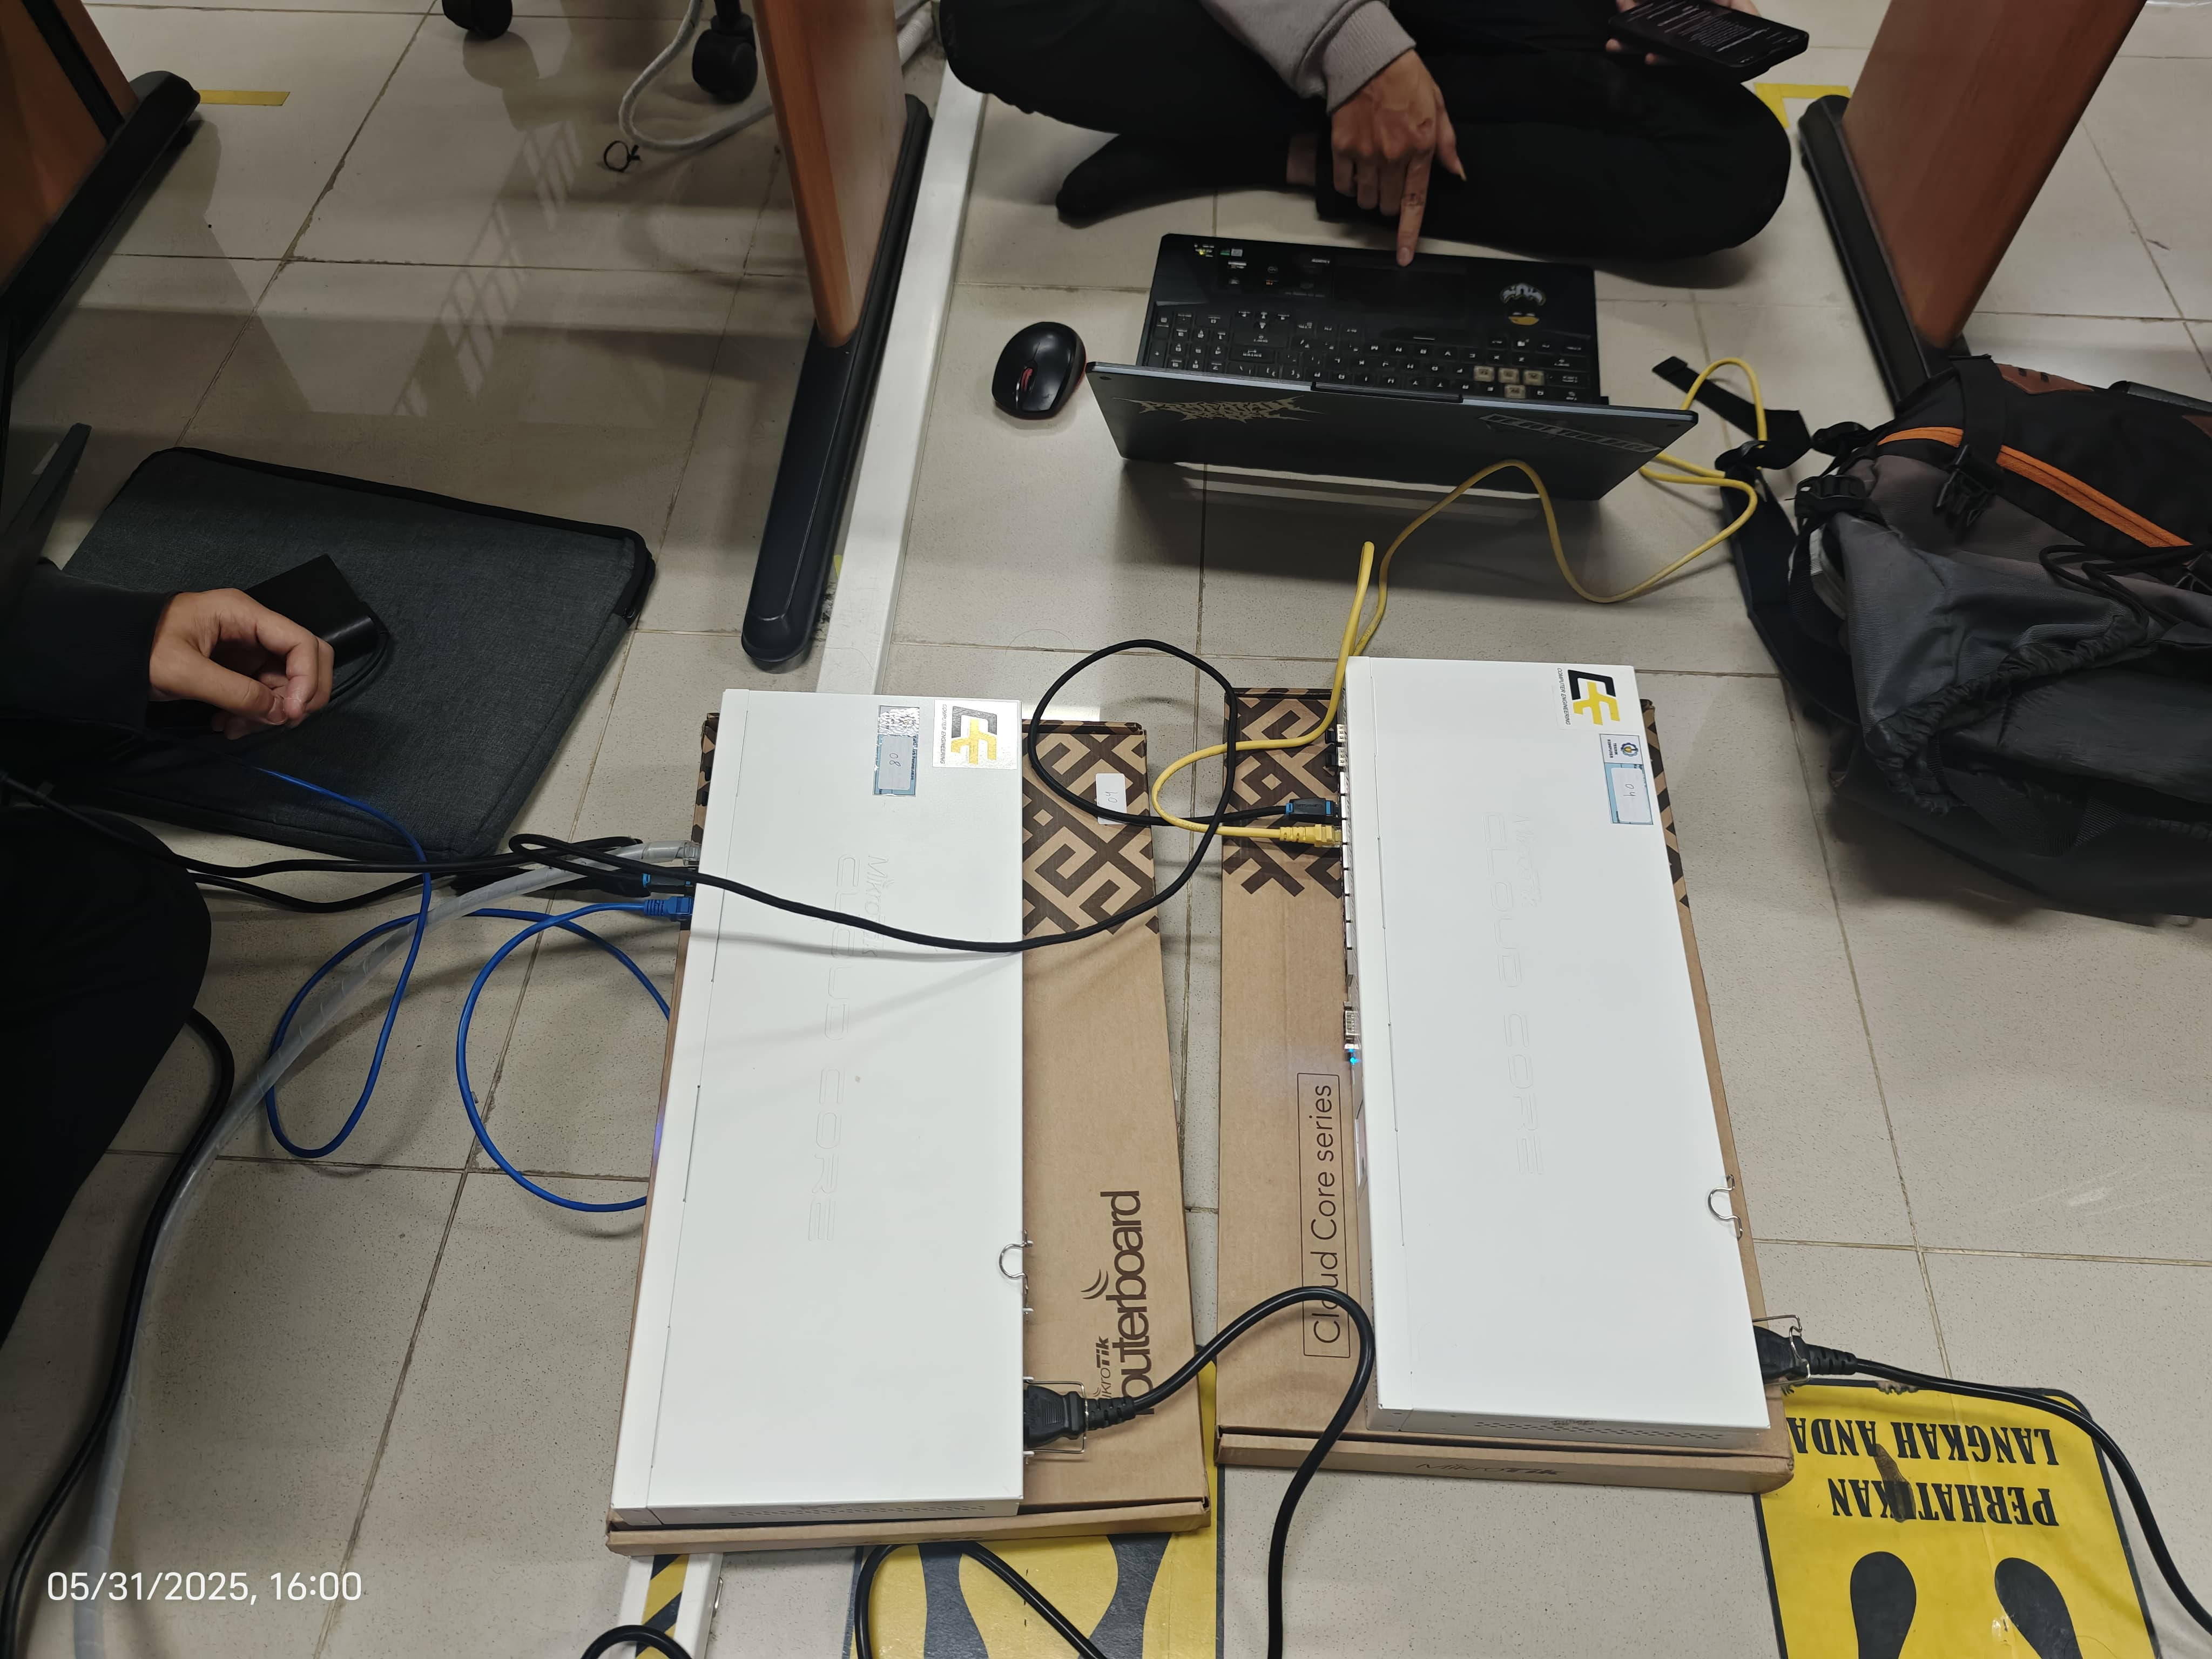
\includegraphics[width=0.4\textwidth]{p4/img/topologi_praktikum.jpg}

